\begin{figure}[h!]
\centering
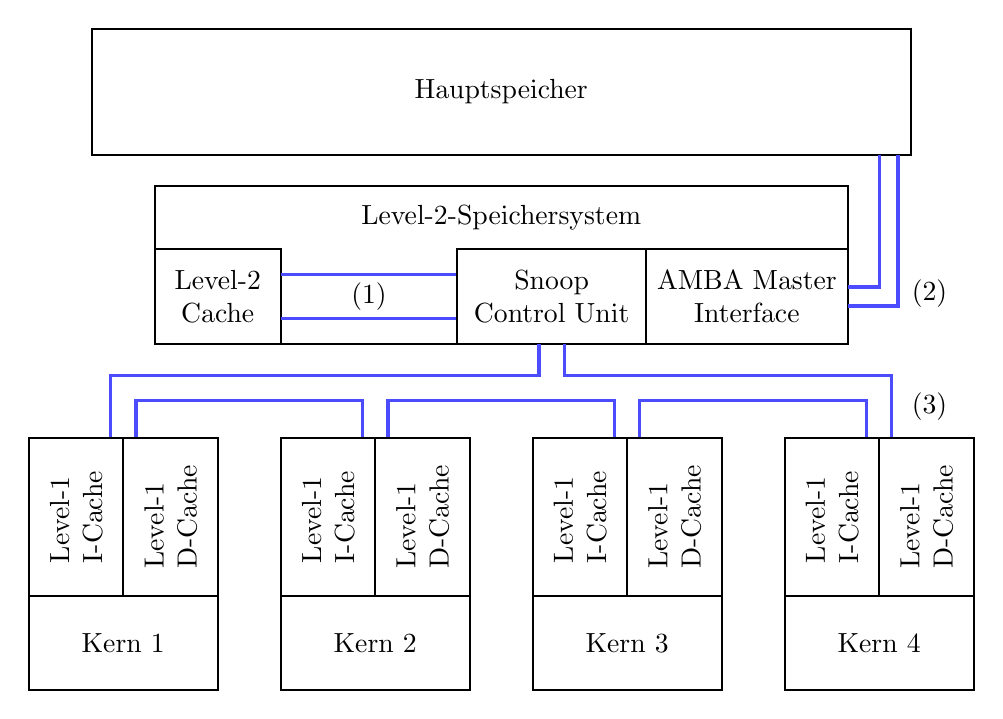
\begin{tikzpicture}[scale=0.8]
	
	% mm
	\draw [thick] (1,16) rectangle (14,14);
	\node at (7.5,15) () {Hauptspeicher};

	% l2-cache
	\draw [thick] (2,13.5) rectangle (13,11);
	\node at (7.5,13) () {Level-2-Speichersystem};
	
	\draw [thick] (9.8,12.5) rectangle (13,11);
	\node [align=center] at (11.4,11.75) () {AMBA Master\\Interface};
	
	\draw [thick] (2,   12.5) rectangle (4,11);
	\node [align=center] at (3,11.75) () {Level-2\\Cache};
		
	\draw [very thick, blue!70] (4,11.4) -- (6.8,11.4);
	\node [align=center] at (5.4,11.75) () {(1)};
	\draw [very thick, blue!70] (4,12.1) -- (6.8,12.1);
	
	\draw [thick] (6.8,12.5) rectangle (9.8, 11);
	\node [align=center] at (8.3,11.75) () {Snoop\\Control Unit};
	
	% SCU to cores
	\draw [very thick, blue!70] (8.1,11) -- (8.1,10.5) -- (1.3,10.5) -- (1.3,9.5);
	\draw [very thick, blue!70] (8.5,11) -- (8.5,10.5) -- (13.7,10.5)-- (13.7,9.5);
	
	\draw [very thick, blue!70] (1.7,9.5) -- (1.7,10.1) -- (5.3,10.1) -- (5.3,9.5);
	\draw [very thick, blue!70] (5.7,9.5) -- (5.7,10.1) -- (9.3,10.1) -- (9.3,9.5);
	\draw [very thick, blue!70] (9.7,9.5) -- (9.7,10.1) -- (13.3,10.1) -- (13.3,9.5);
	\node at (14.3,10) () {(3)};
	
	
	% AMBA to mm
	\draw [very thick, blue!70] (13,11.9) -- (13.5,11.9) -- (13.5,14);
	\draw [very thick, blue!70] (13,11.6) -- (13.8,11.6) -- (13.8,14);
	\node at (14.3,11.8) () {(2)};
	
	% core 1 with l1-cache
	\draw [thick] (0,7) rectangle (3,5.5);
	\node at (1.5,6.25) () {Kern 1};
	\draw [thick] (0,7)   rectangle (1.5,9.5);
	\node[rotate=90,align=left] at (0.75,8.25) () {Level-1\\I-Cache};
	\draw [thick] (1.5,7) rectangle (3,9.5);
	\node[rotate=90,align=left] at (2.25,8.25) () {Level-1\\D-Cache};
	
	% core 2 with l1-cache
	\draw [thick] (4,7)  rectangle (7,5.5);
	\node at (5.5,6.25) () {Kern 2};
	\draw [thick] (4,7)   rectangle (5.5,9.5);
	\node[rotate=90,align=left] at (4.75,8.25) () {Level-1\\I-Cache};
	\draw [thick] (5.5,7) rectangle (7,9.5);
	\node[rotate=90,align=left] at (6.25,8.25) () {Level-1\\D-Cache};
	
	% core 3 with l1-cache
	\draw [thick] (8,7)  rectangle (11,5.5);
	\node at (9.5,6.25) () {Kern 3};
	\draw [thick] (8,7)   rectangle (9.5,9.5);
	\node[rotate=90,align=left] at (8.75,8.25) () {Level-1\\I-Cache};
	\draw [thick] (9.5,7) rectangle (11,9.5);
	\node[rotate=90,,align=left] at (10.25,8.25) () {Level-1\\D-Cache};
	
	% core 4 with l1-cache
	\draw [thick] (12,7)  rectangle (15,5.5);
	\node at (13.5,6.25) () {Kern 4};
	\draw [thick] (12,7)   rectangle (13.5,9.5);
	\node[rotate=90,align=left] at (12.75,8.25) () {Level-1\\I-Cache};
	\draw [thick] (13.5,7) rectangle (15,9.5);
	\node[rotate=90,align=left] at (14.25,8.25) () {Level-1\\D-Cache};
		
\end{tikzpicture}
	\label{memsys}
	\caption{Blockdiagramm des im Raspberry Pi 3b verbauten Cortex A-53 Prozessors  mit den \textcolor{blue!70}{Bussystemen}: (1) Fetch Path ($512 \textrm{ bit}$), (2) AMBA Bus ($128 \textrm{ bit}$), (3) Level-1 Bussysteme mit Leseschnittstelle für Daten und Instruktionen ($128 \textrm{ bit}$) und Schreibschnittstelle für Daten ($256 \textrm{ bit}$)}
\end{figure}
